\documentclass[9pt]{beamer}
\usepackage{threeparttable,url}
\usepackage{dcolumn}
\usepackage{booktabs}
\usepackage{color}
\usepackage{xmpmulti}
\usepackage{animate}
\usepackage{bm}

\definecolor{cobalt}{RGB}{0, 115, 106}
\definecolor{mage}{RGB}{165, 20, 23}

\usepackage[sfdefault]{FiraSans} %% option 'sfdefault' activates Fira Sans as the default text font
\usepackage[T1]{fontenc}
\renewcommand*\oldstylenums[1]{{\firaoldstyle #1}}

\usetheme{metropolis}
%%\setbeamercolor{progress bar}{fg=mage}
%%% \usetheme[pageofpages=of,% String used between the current page and the
%%%                          % total page count.
%%%           bullet=circle,% Use circles instead of squares for bullets.
%%%           titleline=true,% Show a line below the frame title.
%%%           alternativetitlepage=true,% Use the fancy title page.
%%%  %          titlepagelogo=logo-polito,% Logo for the first page.
%%%  %         watermark=watermark-polito,% Watermark used in every page.
%%%           watermarkheight=100px,% Height of the watermark.
%%%           watermarkheightmult=4,% The watermark image is 4 times bigger
%%%                                 % than watermarkheight.
%%%           ]{Torino}

\usepackage{verbatim}
\usepackage{graphicx}
\usepackage{amsmath} 
\usepackage{multirow,multicol}
\usepackage{latexsym}
\usepackage{colortbl,xcolor}
\usepackage{appendixnumberbeamer}
\usepackage{pifont}

% == comment out sections
\usepackage{comment}

% === dcolumn package ===
\usepackage{dcolumn}
\newcolumntype{.}{D{.}{.}{-1}}
\newcolumntype{d}[1]{D{.}{.}{#1}}
\newcommand{\bX}{\mathbf{X}}
\newcommand{\vname}[1]{{\color{mage}{\texttt{#1}}}}
\newcommand{\bone}{\mathbf{1}}

% === Cross out sentences === 
\usepackage[normalem]{ulem}
\newcommand\redsout{\bgroup\markoverwith{\textcolor{red}{\rule[0.5ex]{6pt}{1.5pt}}}\ULon}

% === Multirow cells ===
\usepackage{multirow, booktabs}

% ==== dotted lines in tables ===
\usepackage{arydshln}
\usepackage{threeparttable}
\usepackage{etoolbox}

\usepackage{tcolorbox}

\setbeamercolor{background canvas}{bg=white}

\definecolor{bluegreen}{RGB}{100, 166, 155}
\definecolor{pitchblack}{RGB}{0, 0, 0}
\definecolor{lightbeige}{RGB}{255, 251, 241}
\definecolor{mediumgray}{RGB}{183, 183, 183}
\definecolor{carolinablue}{rgb}{0.0, 0.48, 0.65}
%%\definecolor{cobalt}{rgb}{0.15, 0.38, 0.61}

\setbeamercolor{frametitle}{bg=cobalt, fg=white}
\definecolor{aliceblue}{rgb}{0.74, 0.97, 0.95}

%%\definecolor{cobalt}{rgb}{0.01, 0.31, 0.59}
%%\definecolor{cobalt}{rgb}{0.37, 0.62, 0.63}
%%\definecolor{cobalt}{rgb}{0.21, 0.46, 0.53}
%%\definecolor{cobalt}{RGB}{75, 156, 211}

% === begin document
\begin{document}

\newcommand{\indep}{\mbox{$\perp\!\!\!\perp$}}
\def\independenT#1#2{\mathrel{\rlap{$#1#2$}\mkern2mu{#1#2}}}
% === new commands ===
\newcommand\ud{\mathrm{d}}
\newcommand\dist{\buildrel\rm d\over\sim}
\newcommand\ind{\stackrel{\rm indep.}{\sim}}
\newcommand\iid{\stackrel{\rm i.i.d.}{\sim}}
\newcommand\logit{{\rm logit}}
\renewcommand\r{\right}
\renewcommand\l{\left}

\newcommand{\qs}{q^{\star}}
\newcommand{\E}{\mathbb{E}}
\newcommand{\Var}{\mathrm{Var}}
\newcommand{\Cov}{\mathrm{Cov}}
\newcommand{\tr}{\mathrm{tr}}
\newcommand{\1}{\mathbf{1}}
\newcommand{\const}{\mathrm{const.}}
\newcommand{\bx}{\mathbf{x}}
\newcommand{\tbx}{\tilde{\mathbf{x}}}
\newcommand{\ba}{\mathbf{a}}
\newcommand{\bA}{\mathbf{A}}
\newcommand{\bb}{\mathbf{b}}
\newcommand{\bB}{\mathbf{B}}
\newcommand{\bd}{\mathbf{d}}
\newcommand{\bD}{\mathbf{D}}
\newcommand{\bt}{\mathbf{t}}
\newcommand{\bW}{\mathbf{W}}
\newcommand{\cA}{\mathcal{A}}
\newcommand{\cB}{\mathcal{B}}
\newcommand{\cF}{\mathcal{F}}
\newcommand{\cD}{\mathcal{D}}
\newcommand{\cTN}{\mathcal{TN}}
\newcommand{\balpha}{\boldsymbol{\alpha}}
\newcommand{\bgamma}{\boldsymbol{\gamma}}
\newcommand{\bmu}{\boldsymbol{\mu}}
\newcommand{\bSigma}{\boldsymbol{\Sigma}}
\newcommand{\bbeta}{\boldsymbol{\beta}}
\newcommand{\tbbeta}{\tilde{\boldsymbol{\beta}}}
\newcommand{\xt}{\tilde{x}}
\newcommand{\Tt}{\tilde{\theta}}
\newcommand{\by}{\mathbf{y}}
\newcommand{\bY}{\mathbf{Y}}
\newcommand{\uT}{\underline{T}}
\newcommand{\oT}{\overline{T}}
\newcommand{\fLL}{\texttt{fastLink-L}}
\newcommand{\fLS}{\texttt{fastLink-S}}
\newcommand{\fLdb}{\texttt{fastLink-dblink}}
\newcommand{\fLdbL}{\texttt{fastLink-dblink-L}}
\newcommand{\fLdbS}{\texttt{fastLink-dblink-S}}
\newcommand{\db}{\texttt{dblink}}


\definecolor{cobalt}{RGB}{50, 105,135}

\newcommand{\TedB}{
\includegraphics[height=1.5mm, width = 1.5mm]{./bullet_ted2.png}}
\newcommand{\TedBB}{
\includegraphics[height=1.5mm, width = 1.5mm]{./bullet_ted3.png}}
\newcommand{\TedA}{\textbf{\color{orange} >>}}
\newcommand{\TedC}{\textbf{\color{orange} -}}
\newcommand{\TedD}{\textbf{\color{orange} \Large $\bm{\star}$}}

\setbeamertemplate{itemize items}{\TedA}
\setbeamertemplate{itemize subitem}{\TedB}


\newcommand{\blurb}[1]{\footnotesize \flushleft #1}
\newcommand{\pre}[1]{\texttt{#1}}

%% Multiple slides
\newcounter{multipleslide}

\makeatletter%
\newcommand{\multipleframe}{%
\setcounter{multipleslide}{\value{framenumber}}
\stepcounter{multipleslide}
\patchcmd{\beamer@@tmpl@footline}% <cmd>
  {\insertframenumber}% <search>
  {\themultipleslide}% <replace>
  {}% <success>
  {}% <failure>
}
\newcommand{\restoreframe}{%
\patchcmd{\beamer@@tmpl@footline}% <cmd>
  {\themultipleslide}% <search>
  {\insertframenumber}% <replace>
  {}% <success>
  {}% <failure>
\setcounter{framenumber}{\value{multipleslide}}%
}
\makeatother%

%% R related stuff
\newcommand{\fastLink}{\textsf{fastLink}}
\newcommand{\R}{\textsf{\textbf{R}}}
\newcommand{\Rst}{\textsf{\textbf{RStudio}}}
\newcommand{\code}[1]{\texttt{\color{magenta}{#1}}}

\newcommand\cg{\cellcolor[gray]{0.7}}
\newcommand\cbu{\cellcolor{blue!25}}

\newcommand{\difp}{\hspace{-0.15in}$\rangle$}

\newcolumntype{L}[1]{>{\raggedright\let\newline\\\arraybackslash\hspace{0pt}}m{#1}}
\newcolumntype{C}[1]{>{\centering\let\newline\\\arraybackslash\hspace{0pt}}m{#1}}
\newcolumntype{R}[1]{>{\raggedleft\let\newline\\\arraybackslash\hspace{0pt}}m{#1}}

\newcommand{\argmax}{\operatornamewithlimits{argmax}}
\newcommand{\argmin}{\operatornamewithlimits{argmin}}

\newcommand\spacingset[1]{\renewcommand{\baselinestretch}%
{#1}\small\normalsize}

\newcommand{\arrowT}{$\color{orange} \boldsymbol{\rightsquigarrow}$}

%%\beamerdefaultoverlayspecification{<+->}
\setbeamertemplate{navigation symbols}{}


\title[Probabilistic Blocking]{\Large \color{cobalt} Probabilistic Blocking \\and Distributed Bayesian Entity Resolution}

\author[Ted Enamorado]{{\large{Ted Enamorado \and \hspace{1in} Rebecca C. Steorts\\ {\small Washington University in Saint Louis  \and \hspace{0.2in} Duke University}}} }

\institute[]{{\normalsize }}

\date[]{\medskip {\normalsize } Sept. 23rd, 2020}

%%\section{Title Page}

\begin{frame}[noframenumbering, plain]
\titlepage
\end{frame}


%% -----------------------------------------------------------------------------------------------------------------------------
%% SLIDE 2
%% -----------------------------------------------------------------------------------------------------------------------------

%\begin{frame}
%
%  \frametitle{How We Link Data Sets Matters} 
%
%	\begin{itemize}
%	\item Entity resolution is an increasingly important task across domains (e.g., medicine, 
%	official statistics, human rights, etc)
%	\vfill \pause
%	\item But: How do we link records when a unique identifier is missing?
%	\vfill \pause
%	\begin{itemize}
%	\item {\bf \color{purple} Deterministic methods} e.g., exact matches
%	\begin{itemize}
%			   \item[\TedD] controls false positives 
%			   \pause
%			   \item[$\rightsquigarrow$] not robust to {\bf {typographical errors}} and {\bf {missing values}}  
%	\end{itemize}		   
%	\vfill \pause  
%	\item {\bf \color{purple} Probabilistic Record Linkage (PRL)} 
%		\begin{itemize}
%			   \item[\TedD] designed to control error rates  \pause
%			   	\smallskip\smallskip
%			   \item[$\rightsquigarrow$] existing open-source implementations need to scale to billions of records \\  \pause
%			    \TedD\ \texttt{fastLink}  (Enamorado et al., 2019) \\
%			    \TedD\ \texttt{dblink}  (Marchant et al., 2020) \\	
%			     \TedD\ \texttt{dblinkR}  (Marchant et al., 2020) \\
%			    		    \pause
%			   	\smallskip\smallskip
%			   \item[$\rightsquigarrow$] providing accuracy to two-stage blocking and linkage procedures \\  \pause
%			    \TedD\ This project: \texttt{fastLink} (blocking) + \texttt{dblink} (linkage)
%	 \end{itemize}
%	 \end{itemize}
%	\end{itemize}
%
%\end{frame}

\frame{

\Large
\center
Entity resolution is the process of merging large noisy databases to remove duplicate entities , often in the absence of a unique identifier. 


}

\frame{

\Large
\center
This problem is fundamentally important in medicine, official statistics, human rights and modern slavery, voter registration, and many other applications. 

}

\frame{
\frametitle{Background}

\Large
\center
Deterministic methods are very popular as they are easily accessible across multiple disciplines and very scalable. 

\vspace*{1em}

They do not account for the error of the entity resolution process. 

\vspace*{1em}

Binette and \textbf{Steorts} (2020), Under Review 


}

\frame{
\frametitle{Probabilistic Entity Resolution}


\begin{itemize}
\item Designed to control error rates (precision and recall)
\item Designed to model data with distortions and errors
\end{itemize}
\pause

Existing open-source implementations need to scale to billions of records \\  \pause
\begin{enumerate}
\item[{\color{orange} \bf 1.}]  \texttt{fastLink}  (Enamorado et al., 2019) \\
\item[{\color{orange} \bf 2.}]  \texttt{dblink}  (Marchant et al., 2020) \\	
\item[{\color{orange} \bf 3.}] \texttt{dblinkR}  (Marchant et al., 2020) \\
\end{enumerate} 

Our goal is to propose a two-stage method that will scale and have a balance regarding uncertainty propagation. This is called: 

\texttt{fastLink} (blocking) + \texttt{dblink} (linkage)

\vspace*{1em}

\textbf{Enamorado} and \textbf{Steorts} (2020), PSD



}



%% -----------------------------------------------------------------------------------------------------------------------------
%% TRANSITION
%% -----------------------------------------------------------------------------------------------------------------------------

\begin{frame}[plain]
\frametitle{Road to Improving Probabilistic Entity Resolution}

\begin{itemize}
\item[{\color{orange} \bf 1.}] fastLink
\vfill
\item[{\color{orange} \bf 2.}] dblink 
\vfill
\item[{\color{orange} \bf 3.}] fastLink + dblink 
\vfill
\item[{\color{orange} \bf 4.}] Results: 
\vfill
\begin{itemize}
\item[\TedB] Validation Study: \texttt{RLdata10000}  \vfill
\item[\TedB] Empirical Application: National Long Term Care Study (\texttt{NLTCS})
\end{itemize}
\vfill
\end{itemize}
\end{frame}

\begin{frame}[plain]
\frametitle{Road to Improving Probabilistic Entity Resolution}

\begin{itemize}
\item[{\color{orange} \bf 1.}] fastLink
\vfill
\item[{\color{orange!30} \bf 2.}] {\color{black!30} dblink }
\vfill
\item[{\color{orange!30} \bf 3.}] {\color{black!30} fastLink + dblink }
\vfill
\item[{\color{orange!30} \bf 4.}] {\color{black!30} Results: }
\vfill
\begin{itemize}
\item[\TedBB] {\color{black!30} Validation Study: \texttt{RLdata10000} } \vfill
\item[\TedBB] {\color{black!30} Empirical Application: National Long Term Care Study (\texttt{NLTCS})}
\end{itemize}
\vfill
\end{itemize}
\end{frame}

\addtocounter{framenumber}{-2}


%% -----------------------------------------------------------------------------------------------------------------------------
%% SLIDE
%% -----------------------------------------------------------------------------------------------------------------------------

\begin{frame}
  \frametitle{Agreement Patterns}
  \vspace{3mm}
\begin{overlayarea}{\textwidth}{\textheight}
\only<1-3>{
\begin{itemize}
\only<1-3>{\item Two data sets ($\cA$ and $\cB$) with variables in common}
\only<2-3>{\item Agreement value in field $a$ for a pair $(i,j)$
    $$\rho_a(i,j) \ = \ \left\{\begin{array}{l}   \color{blue}{\texttt{agree}} \\ \\
    								     \color{blue}{\texttt{disagree}} \end{array}
                               \right. $$
\begin{tabular}{ccccccc}
    &  & \multicolumn{2}{c}{Name} & \multicolumn{1}{c}{} & \multicolumn{1}{c}{} \\ \cmidrule(lr){3-4}  
    &  & First & Last &  Age & Street \\ 
  \hline
    & \multicolumn{3}{l}{Data set $\mathcal{A}$} \\
    &  1 &  \texttt{James}  	& \texttt{Smith}  	& \texttt{35} & \bf{{\texttt{Devereux St.}}} \\
    &  \multicolumn{3}{l}{Data set $\mathcal{B}$} \\
    &  7 &  \texttt{James} 	& \texttt{Smit} 		& \texttt{43} & \bf{{\texttt{Dvereux St.}}}  \\ 
	 \hdashline
    & & \color{blue} {\texttt{agree}} 	& \color{blue} {\texttt{agree}}  	& \color{blue} {\texttt{disagree}} 		&   \color{blue} {\bf{{\texttt{agree}}}} \\  \hline
\end{tabular}
}

\only<3-3>{
\vspace{4mm}
\begin{tcolorbox}[colback= {white},colframe= {cobalt},title={}]
{
\begin{center}
\textbf{Agreement pattern} $\rho(i, j) = \{\rho_1(i,j), \rho_2(i,j), \ldots, \rho_K(i,j) \}$ 
\end{center}  
} 
\end{tcolorbox}
}
\end{itemize}
}
\end{overlayarea}

\end{frame}


%% -----------------------------------------------------------------------------------------------------------------------------
%% SLIDE
%% -----------------------------------------------------------------------------------------------------------------------------

\begin{frame}
\frametitle{The Fellegi-Sunter Model of PRL}
 
  \begin{itemize}
	 \item \textbf{We observe} the agreement patterns $\gamma(i, j)$ 
	 \item \textbf{We do not observe} the matching status

           $$C(i,j) \ = \ \left\{ \begin{array}{cl} 
           				\text{\color{blue}{non-match}}  \\ 
                                          \text{\color{red}{match}} 
                                          \end{array} \r.$$ \pause
\begin{tcolorbox}[colback=blue!0,colframe={cobalt},title= {\bf Mixture Model}]
{\small 
\begin{center}
\begin{eqnarray*}
  C(i, j) & \iid & \text{Bernoulli}(\mu) \\ 
  \rho(i,j) \mid C(i, j) = \text{\color{blue}{non-match}} & \iid &  \mathcal{F}({ \color{blue}{\pi}_{\text{\color{blue}{NM}}} }) \\ 
  \rho(i,j) \mid C(i, j) = \text{\color{white}{non-}\color{red}{match}} & \iid &  \mathcal{F}( {\color{red}{\pi}_{\text{\color{red}{M}}} }) 
\end{eqnarray*} 
\end{center}
}  
\end{tcolorbox}
  \item Where 
  {\normalsize $\lambda$, ${\color{red}{\pi}_{\text{\color{red}{M}}}}$, ${\color{blue}{\pi}_{\text{\color{blue}{NM}}}}$  are estimated via the EM algorithm} 
  \end{itemize}

\end{frame}

%% -----------------------------------------------------------------------------------------------------------------------------
%% SLIDE
%% -----------------------------------------------------------------------------------------------------------------------------

\begin{frame}
\frametitle{Runtime Comparison}

\vspace{-1mm}
  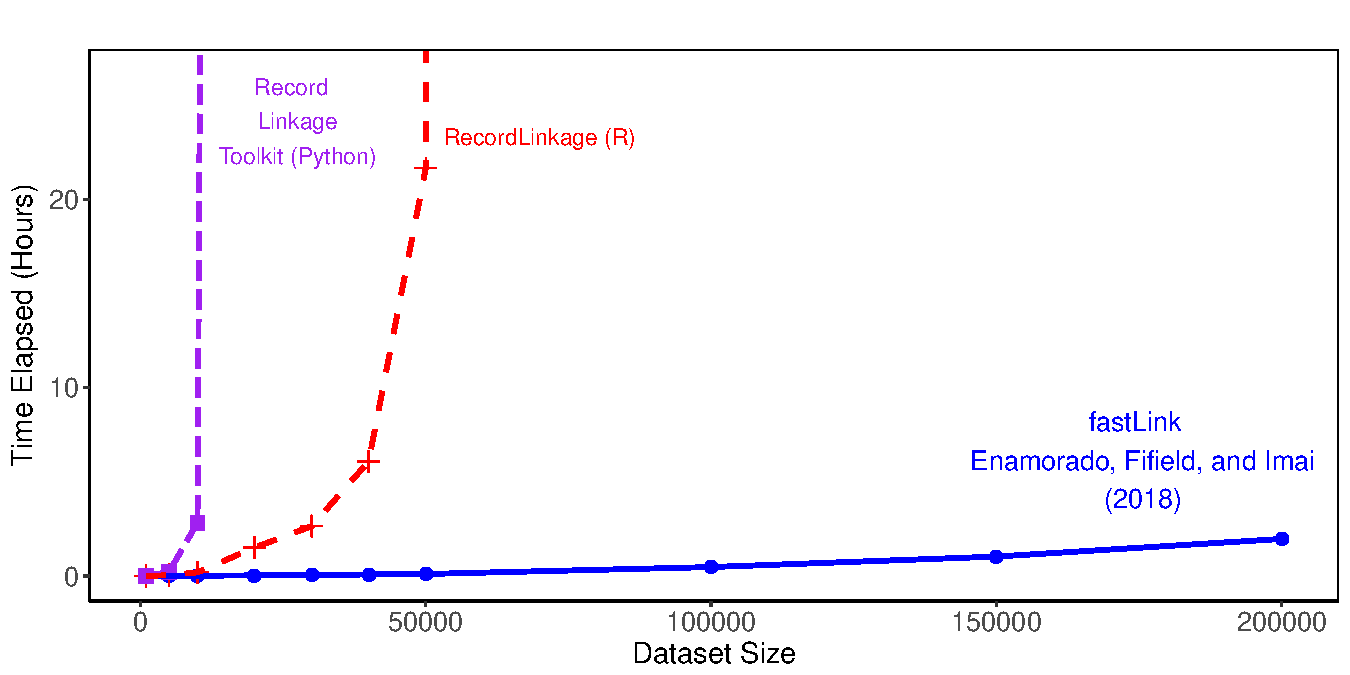
\includegraphics[width=\linewidth,height=\textheight,keepaspectratio]{./figs/runtime_overall.pdf} 
\vspace{-6mm}
    \begin{itemize}
  \item Data sets of equal size
  \item Variables in common: first and last name; house number, street name and zip code; age \pause
  \item \textbf{Key:} \code{Sparse matrix} representation of a \code{hash table}
  \item[]
  \item[] \textbf{Enamorado}, Fifield, and Imai (2019), APSR, In Press
  \end{itemize}
\end{frame}
%% -----------------------------------------------------------------------------------------------------------------------------
%% TRANSITION
%% -----------------------------------------------------------------------------------------------------------------------------

\begin{frame}[plain]
\frametitle{Road to Improving Probabilistic Entity Resolution}

\begin{itemize}
\item[{\color{orange!30} \bf 1.}] {\color{black!30} fastLink}
\vfill
\item[{\color{orange} \bf 2.}] dblink
\vfill
\item[{\color{orange!30} \bf 3.}] {\color{black!30} fastLink + dblink }
\vfill
\item[{\color{orange!30} \bf 4.}] {\color{black!30} Results: }
\vfill
\begin{itemize}
\item[\TedBB] {\color{black!30} Validation Study: \texttt{RLdata10000} } \vfill
\item[\TedBB] {\color{black!30} Empirical Application: National Long Term Care Study (\texttt{NLTCS})}
\end{itemize}
\vfill
\end{itemize}
\end{frame}

\addtocounter{framenumber}{-1}


%% -----------------------------------------------------------------------------------------------------------------------------
%% SLIDE
%% -----------------------------------------------------------------------------------------------------------------------------

\begin{frame}
\frametitle{Distributed end-to-end Bayesian Entity Resolution (dblink)}

\begin{itemize}
\item The goal of dblink:
\vfill
\item[] Scaling Bayesian ER methods to millions of records without  sacrificing accuracy
   and crucially giving uncertainty of the ER task 
\vfill   
\item[]   Marchant, Kaplan, Elzar, Rubinstein, \textbf{Steorts} (2020), JCGS, In Press
\end{itemize} 
\vfill

\end{frame}

%% -----------------------------------------------------------------------------------------------------------------------------
%% SLIDE
%% -----------------------------------------------------------------------------------------------------------------------------

\begin{frame}
\frametitle{Distributed end-to-end Bayesian Entity Resolution}

\begin{enumerate}
\item[{\color{orange} \bf 1.}] Proposing the first joint blocking and entity resolution model that scales to millions of records. \vfill
\item[{\color{orange} \bf 2.}] Utilizes auxiliary partitions (blocks) that induce conditional independencies between latent entities, which enables  distributed inference at the partition-level. \vfill
\item[{\color{orange} \bf 3.}] A blocking function (responsible for partitioning the entities), which groups similar entities together while achieving well-balanced partitions. \vfill
\item[{\color{orange} \bf 4.}] Application of partially-collapsed Gibbs sampling in the context of distributed computing. \vfill
\item[{\color{orange} \bf 5.}] Improving the overall computational efficiency. \vfill
\item[{\color{orange} \bf 6.}] Applying the proposed methodology to six synthetic and real data sets, including a case study of the 2010 decennial census. \vfill
\item[{\color{orange} \bf 7.}] Open source code available in Apache Spark and R. \vfill
\end{enumerate}

%\begin{enumerate}
%\item Incorporating auxiliary partitions that
%induce conditional independencies between the entities. This enables distributed inference at the partition-level, while crucially preserving the marginal posterior of the original model. 
%\item A partition function (responsible for partitioning the entities), which groups similar entities together while achieving well-balanced partitions.
%\item Application of partially-collapsed Gibbs sampling in the context of distributed computing.
%\item Improving computational efficiency:
%\begin{enumerate}
%\item[a)] Sub-quadratic algorithm for updating links based on indexing.
%\item[b)] Truncation of the attribute similarities.
%\item[c)] Perturbation sampling algorithm for updating the entity attributes, which relies on the Vose-Alias method.
%\end{enumerate}

 \vspace*{1em} 
   
   Marchant, Kaplan, Elzar, Rubinstein, \textbf{Steorts} (2020), JCGS, In Press
 
\end{frame}

%% -----------------------------------------------------------------------------------------------------------------------------
%% SLIDE
%% -----------------------------------------------------------------------------------------------------------------------------

\begin{frame}
\frametitle{Distributed end-to-end Bayesian Entity Resolution}
 
 \vspace{3mm}
 \begin{center}
  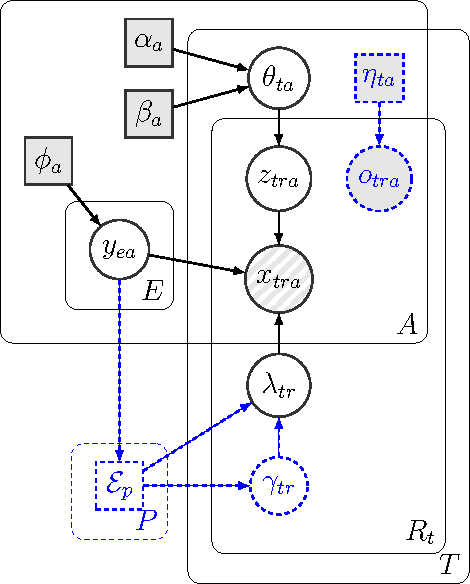
\includegraphics[width=\linewidth,height=0.85\textheight,keepaspectratio]{./figs/plate-diagram2.pdf} 
 \end{center}
\end{frame}

%% -----------------------------------------------------------------------------------------------------------------------------
%% TRANSITION
%% -----------------------------------------------------------------------------------------------------------------------------

\begin{frame}[plain]
\frametitle{Road to Improving Probabilistic Entity Resolution}

\begin{itemize}
\item[{\color{orange!30} \bf 1.}] {\color{black!30} fastLink}
\vfill
\item[{\color{orange!30} \bf 2.}] {\color{black!30} dblink}
\vfill
\item[{\color{orange} \bf 3.}] {\color{black} fastLink + dblink }
\vfill
\item[{\color{orange!30} \bf 4.}] {\color{black!30} Results: }
\vfill
\begin{itemize}
\item[\TedBB] {\color{black!30} Validation Study: \texttt{RLdata10000} } \vfill
\item[\TedBB] {\color{black!30} Empirical Application: National Long Term Care Study (\texttt{NLTCS})}
\end{itemize}
\vfill
\end{itemize}
\end{frame}

\addtocounter{framenumber}{-1}


%% -----------------------------------------------------------------------------------------------------------------------------
%% SLIDE
%% -----------------------------------------------------------------------------------------------------------------------------

\begin{frame}
\frametitle{\fLdb}

\begin{itemize}
\item We propose a two-stage approach that combines the strengths of \texttt{fastLink} and \texttt{dblink} where:
\vfill
\begin{itemize}
\item[{\color{orange} \bf 1.}]  Instead of resorting to traditional blocking strategies we use \texttt{fastLink} to look for potential matches
\vfill
\item[{\color{orange} \bf 2.}]  We use \texttt{dblink} to determine the co-reference structure of the linkages
\vfill
\end{itemize}
\item \texttt{fastLink} provides fast blocking and \texttt{dblink} provides exact uncertainty propagation
\end{itemize}
\end{frame}

%% -----------------------------------------------------------------------------------------------------------------------------
%% TRANSITION
%% -----------------------------------------------------------------------------------------------------------------------------

\begin{frame}[plain]
\frametitle{Road to Improving Probabilistic Entity Resolution}

\begin{itemize}
\item[{\color{orange!30} \bf 1.}] {\color{black!30} fastLink}
\vfill
\item[{\color{orange!30} \bf 2.}] {\color{black!30} dblink}
\vfill
\item[{\color{orange!30} \bf 3.}] {\color{black!30} fastLink + dblink }
\vfill
\item[{\color{orange} \bf 4.}] {\color{black} Results: }
\vfill
\begin{itemize}
\item[\TedB] {\color{black} Validation Study: \texttt{RLdata10000} } \vfill
\item[\TedBB] {\color{black!30} Empirical Application: National Long Term Care Study (\texttt{NLTCS})}
\end{itemize}
\vfill
\end{itemize}
\end{frame}

\addtocounter{framenumber}{-1}

%% -----------------------------------------------------------------------------------------------------------------------------
%% SLIDE
%% -----------------------------------------------------------------------------------------------------------------------------

\begin{frame}
\frametitle{\texttt{RLdata10000}}
 
\begin{itemize}
\item Validation based on \texttt{RLdata10000} from the R-package \texttt{RecordLinkage}
\vfill
\item It contains 10\% duplicates
\vfill
\item Linkage fields include: first and last name; day, month, and year of birth
\vfill
\item For \fLdb\ we consider two blocking approaches: loose (FDR < 10\%) and strict  (FDR < 1\%)
\vfill
\end{itemize}
 
\end{frame}

\begin{frame}
\frametitle{Results }
 
 
\begin{table}[h!]
	\centering
	\caption{Comparison of Matching Quality.
		``ARI'' stands for adjusted Rand index and ``Err. \# clust.'' 
		is the percentage error in the number of clusters.}
	\label{tbl:linkage-quality}
	\footnotesize
	\begin{tabular}{l l *{5}{c}}
		\toprule
		Dataset    & Method & \multicolumn{3}{c}{Pairwise measures} & \multicolumn{2}{c}{Cluster measures} \\
		\cmidrule(lr){3-5} \cmidrule(lr){6-7}
		& & Precision & Recall & F1-score & ARI & Err. \# clust.\ \\
		\midrule
		\multirow{5}{*}{\texttt{RLdata10000}}
		& dblink              & 0.63 & 1.00 & 0.78 & 0.78 & --10.97\% \\
		& \fLL   & 0.94	& 0.98	& 0.96 & --- & --- \\\
		& \fLS   &  0.96 & 0.98 & 0.97 & --- & --- \\
		& \fLdbL   & 0.94 & 1.00 & 0.97 & 0.97 & -0.34\% \\
		& \fLdbS    & 0.96 &  1.00 &  0.98 & 0.98 & -0.17\% \\
		\bottomrule
	\end{tabular}
\end{table}
 
\end{frame}

%% -----------------------------------------------------------------------------------------------------------------------------
%% TRANSITION
%% -----------------------------------------------------------------------------------------------------------------------------

\begin{frame}[plain]
\frametitle{Road to Improving Probabilistic Entity Resolution}

\begin{itemize}
\item[{\color{orange!30} \bf 1.}] {\color{black!30} fastLink}
\vfill
\item[{\color{orange!30} \bf 2.}] {\color{black!30} dblink}
\vfill
\item[{\color{orange!30} \bf 3.}] {\color{black!30} fastLink + dblink }
\vfill
\item[{\color{orange} \bf 4.}] {\color{black} Results: }
\vfill
\begin{itemize}
\item[\TedBB] {\color{black!30} Validation Study: \texttt{RLdata10000} } \vfill
\item[\TedB] {\color{black} Empirical Application: National Long Term Care Study (\texttt{NLTCS})}
\end{itemize}
\vfill
\end{itemize}
\end{frame}

\addtocounter{framenumber}{-1}

%% -----------------------------------------------------------------------------------------------------------------------------
%% SLIDE
%% -----------------------------------------------------------------------------------------------------------------------------

\begin{frame}
\frametitle{\texttt{NLTCS}}
 
\begin{itemize}
\item \texttt{NLTCS} is a longitudinal study of health and well-being of those in the U.S. older than 65
\vfill
\item 3 waves, which account for 57,077 observations
\vfill
\item Hard test: data has been anonymized. Can we recover the true linkage structure?
\vfill
\item Linkage fields: full date of birth, state, location of doctor's office, and gender
\vfill
\item The number of unique individuals in the data is 34,945
\end{itemize}
 
\end{frame}

\begin{frame}
\frametitle{Results }
 
 \begin{table}[h!]
	\centering
	\caption{Comparison of matching quality.
		``ARI'' stands for adjusted Rand index and ``Err. \# clust.'' 
		is the percentage error in the number of clusters.}
	\label{tbl:linkage-quality-real}
	\footnotesize
	\begin{tabular}{l l *{5}{c}}
		\toprule
		Dataset    & Method & \multicolumn{3}{c}{Pairwise measures} & \multicolumn{2}{c}{Cluster measures} \\
		\cmidrule(lr){3-5} \cmidrule(lr){6-7}
		& & Precision & Recall & F1-score & ARI & Err. \# clust.\ \\
		\midrule
		\multirow{5}{*}{\texttt{NLTCS}}
		& dblink              & 0.83 & 0.91 & 0.87 & 0.87 & --22.09\% \\
		& \fLL   &  0.80	& 0.91	& 0.80 & --- & --- \\
		& \fLS   & 0.91 &	0.91	& 0.91 & --- & --- \\
		& \fLdbL  &     0.87 & 0.94 & 0.90 & 0.90 & -13.01\% \\
		& \fLdbS    &   0.91  & 1.00 & 0.95 & 0.95 & 2.79\% \\
		\bottomrule
	\end{tabular}
\end{table}

 
\end{frame}

%% -----------------------------------------------------------------------------------------------------------------------------
%% SLIDE
%% -----------------------------------------------------------------------------------------------------------------------------

\begin{frame}
\frametitle{Concluding Remarks}

\begin{itemize}
\item Motivated by the need to scale ER to large data sets (in fast and accurate ways) we have proposed a 
two-stage approach to blocking and ER.
\vfill
\item \fLdb\ is an open-source pipeline that could be useful for applied researchers on how to improve their
own
\vfill 
\item There are lots of opportunities to improve upon \fLdb\ e.g., automating the pipeline
\vfill
\item As always, we recommend caution when using ER methods so that personal privacy is never at risk.
\vfill
\end{itemize}

\end{frame}

%% -----------------------------------------------------------------------------------------------------------------------------
%% SLIDE
%% -----------------------------------------------------------------------------------------------------------------------------

\begin{frame}
\frametitle{Computational Complexity of \fLdb\ }

\begin{itemize}
\item Assume without loss of generality that each dataset is of equal size $N$ \vfill
\item Let $N_{max}$ represent the total number of records in all databases \vfill
\item Let $N^{\ast}_{max} \ll N_{max}$ is the number of records classified as possible matches by fastLink \vfill
\item Let $S_G$ denote the total number of MCMC iterations \vfill
\item {\bf Theorem:} The computational complexity of \fLdb\ is $$O(\Upsilon N_{max}  (N_{max} - 1)) + O(S_G N^\ast_{max}), \quad \text{where} \quad \Upsilon  = \frac{\omega}{2Q}.$$
where $\omega$ represents the share of unique values per linkage field and $Q$ the number of threads available on your computer
\end{itemize}
 \vfill
\end{frame}


%% -----------------------------------------------------------------------------------------------------------------------------
%% SLIDE
%% -----------------------------------------------------------------------------------------------------------------------------

\begin{frame}
\frametitle{Appendix}

\begin{itemize}
\item Convergence rates: Number of unique entities in \texttt{RLdata10000}
\begin{center}
  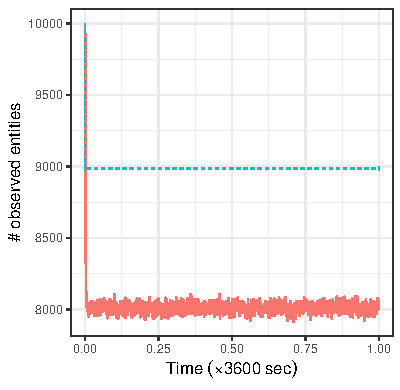
\includegraphics[width=\linewidth,height=0.8\textheight,keepaspectratio]{./figs/convergence-num-ent-blink-dblink-rldata10000.pdf} 
\end{center}
\end{itemize}
\end{frame}

\begin{frame}
\frametitle{Appendix}

\begin{itemize}
\item Convergence rates: Number of unique entities in \texttt{NLTCS}
\begin{center}
  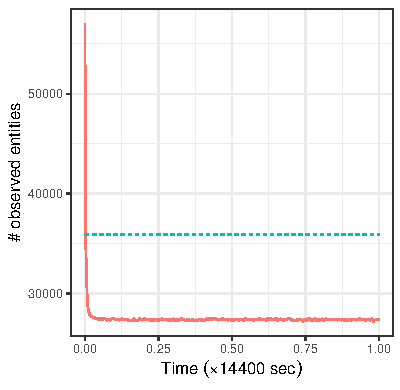
\includegraphics[width=\linewidth,height=0.8\textheight,keepaspectratio]{./figs/convergence-num-ent-blink-dblink-nltcs.pdf} 
\end{center}
\end{itemize}

\end{frame}


\end{document}

